\section{Main Services}
\label{sec:main_services}
The next sections explain the three main services, namely \acl{hcs} (section \ref{sec:hooks_checking_service}), \acl{jms} (section \ref{sec:jobs_managing_service}), and \acl{tbs} (section \ref{sec:ts_benchmarking_service}).

This explanation follows the flow of actions that happen while a user is configuring a continuous benchmark and the process that happens when a benchmark is initiated.

The explanations are based on provided diagrams, code review and analysis, and information provided by former developers of the project.
\\

Figure \ref{fig:basilisk_high_level_design_approach} gives an overview of the three microservices of the Basilisk platform.
It shows the most important messages send between the services and the interactions with \gh{} and \dockh{}.
\begin{figure}[tbph]
	\centering
	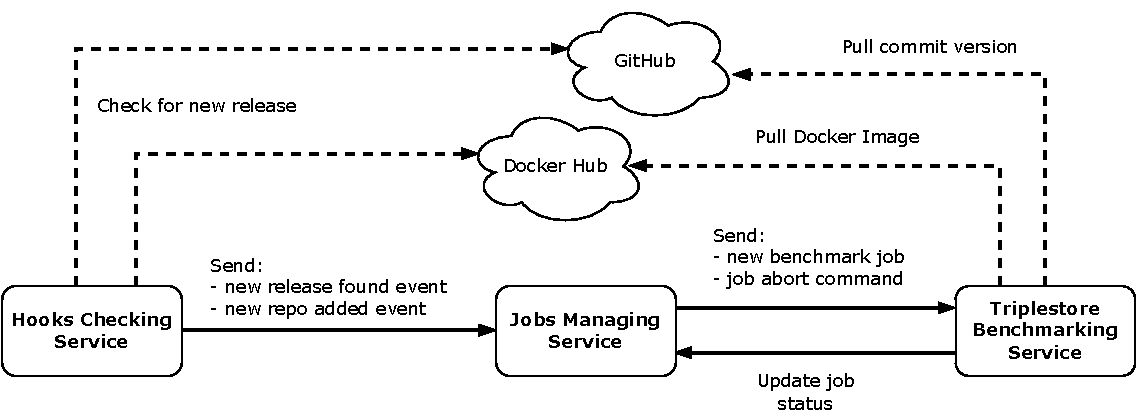
\includegraphics[width=1\textwidth]{figures/high-level-design-approach.pdf}
	\caption{Overview of the three microservices}
	\label{fig:basilisk_high_level_design_approach}
\end{figure}



\subsection{\acl{hcs}}
\label{sec:hooks_checking_service}
The main task of the \ac{hcs} is to observe \gh{} and \dockh{} repositories of \tsp{} for new releases or changes.

When a user wants to set up a new continuous benchmark, the \ac{hcs} needs to be informed which repository (\gh{} or \dockh{}) has to be observed for changes.
This happens through REST API calls to the \ac{hcs} providing the repository name and owner.
The \ac{hcs} will then create a hook for the repository to get notice about changes.
A hook is in general a piece of code or software that attaches itself to a software component to intercept messages and react to those messages, \eg, with function calls.
In the case of the \ac{hcs} the hooks can be seen as bookmarks for the repositories.
Each hook stores the latest known version of an repository.
The service will query the saved repositories regularly and compare their current version to the version stored in the hook.

When the \ac{hcs} notices a new release for a repository, it updates the corresponding hook to the newest version.
Then it sends a message about the new version to the \aclp{jrq} from which the \acl{jms} retrieves the message.

\subsubsection{API and Messaging}
\label{sec:hooks_api}
The \ac{hcs} is controlled by the user over a REST API.

The continuous checking of the repositories can be started and stopped over a REST endpoint.
The other most important endpoints are for adding and deleting \gh{} and \dockh{} repositories.
Figure \ref{fig:rest_apis_approach_hcs} shows these endpoints.
\begin{figure}[tbph]
	\centering
	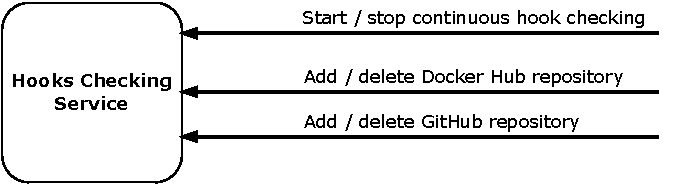
\includegraphics[width=.57\textwidth]{figures/rest-apis-approach-hcs.pdf}
	\caption{REST API of the \acl{hcs}}
	\label{fig:rest_apis_approach_hcs}
\end{figure}

The communication between the \ac{hcs} and the \acl{jms} is done over RabbitMQ (\ref{sec:rabbitmq}) messages, over the \aclp{jrq}.
The messages contain different events that can occur in the \ac{hcs}.
For example an event is send when adding or deleting a repository, or a new release is detected.


\subsection{\acl{jms}}
\label{sec:jobs_managing_service}
The main task for the \acf{jms} is to create benchmark jobs, when a new release was found by the \ac{hcs}.
Other important functionality of the \ac{jms} is the management of the configurations needed for the benchmarks.
Lastly the \ac{jms} manages the status for running and pending jobs send to the \acl{tbs}.
\\

There are three configuration types needed for a benchmark job.
First the platform needs the configuration for the \ts{}.
This configuration includes for example the SPARQL endpoint as well as the user and password for the connection to the endpoint.
This is needed by the \iguana{} framework to properly connect to the \ts{} under test\cite{IguanaDocumentationConfiguration}.

Secondly the platform needs configurations for datasets and query files.
The dataset configuration simply consists of the dataset name and the URL for the location of the dataset.
The query configuration consists similarly of a name for the queries and the URL for the location of the query file.

These configurations are added over the REST API of the \ac{jms}.
\\

When the \ac{hcs} sends an event regarding a new release of a repository, the \ac{jms} will create benchmark jobs for the new release.
A benchmark job consists of the current version of the repository, a query configuration and a dataset.
For each event multiple benchmark jobs can be created.
For each query configuration and dataset one benchmark job will be created.

These benchmark jobs will then be send to the \acl{tbs} over the \acl{bjq}.

The management of the running and pending benchmark jobs is done over the REST API of the \ac{jms}.
When an endpoint is triggered, \eg, to abort a pending job, the \ac{jms} sends an event to the \acl{tbs}.


\subsubsection{API and Messaging}
\label{sec:jobs_api}
The \ac{jms} communicates with the \ac{hcs} and the \acl{tbs} over RabbitMQ message queues.
The service receives repository events from the \ac{hcs} and sends benchmark job events to the \acl{tbs} over the \ac{bjq}.
\\

Interaction of the user is handled over the REST API.
The API offers endpoints for adding and deleting the different configurations of \tsp{}, datasets and queries
A second set of endpoints are for querying the job status of running and pending jobs, and for stopping individual jobs.
Figure \ref{fig:rest_apis_approach_jms} shows these endpoints.
\begin{figure}[tbph]
	\centering
	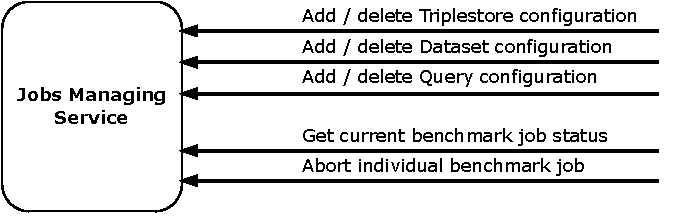
\includegraphics[width=.57\textwidth]{figures/rest-apis-approach-jms.pdf}
	\caption{REST API of the \acl{jms}}
	\label{fig:rest_apis_approach_jms}
\end{figure}


\subsection{\acl{tbs}}
\label{sec:ts_benchmarking_service}
The \ac{tbs} executes the benchmark jobs send by the \ac{jms} and saves the benchmark results to the \acl*{jsts}.

To execute a benchmark the service needs a running instance of the \ts{} under test on which the benchmark will be executed.
This instance is build from the information and configurations provided in the benchmark job.
The \ac{tbs} will query the provided repository (\gh{} or \dockh{}) for the version specified in the job.

If the repository is from \gh{}, the \ac{tbs} downloads the source code for the provided commit and searches for a Dockerfile.
It then builds and runs a Docker container from that Dockerfile.

If the repository is from \dockh{}, the \ac{tbs} pulls the image with the provided tag.
It then runs the image as a Docker Container.
\\

After starting the Docker Container the \ac{tbs} starts the \iguana{} framework.
\iguana{} will perform the benchmark with the provided configuration from the benchmark job.

When the benchmark is finished the results are written to the \acl*{jsts}

\subsubsection{API and Messaging}
\label{sec:benchmarking_api}
The \ac{tbs} has no REST API.
The service is controlled through the \ac{jms} by events send over RabbitMQ.

The events received from the \ac{jms} are new benchmark jobs and pause or abort commands for running benchmark jobs.
The \ac{tbs} sends short events containing the status of benchmark jobs, \eg, a job has started, or it has finished and the results are uploaded to the \acl{jsts}.